% Consistent but Blind? -- term project report (computer vision course, 2026)
% Compile with pdfLaTeX + BibTeX (e.g. upload the report/ folder to Overleaf).
\documentclass[10pt,twocolumn,letterpaper]{article}

\usepackage[T1]{fontenc}
\usepackage{mathptmx}
\usepackage[margin=0.75in,columnsep=0.3in]{geometry}
\usepackage{graphicx}
\usepackage{booktabs}
\usepackage{amsmath,amssymb}
\usepackage{xcolor}
\usepackage[numbers,sort&compress]{natbib}
\usepackage[colorlinks=true,linkcolor=blue!50!black,citecolor=blue!50!black,urlcolor=blue!50!black]{hyperref}
\usepackage[font=small,labelfont=bf]{caption}
\usepackage{enumitem}
\setlist{nosep,leftmargin=1.2em}

\usepackage{xspace}
% Abbreviations as in the CVPR template: no double period at the end of a sentence.
\makeatletter
\DeclareRobustCommand\onedot{\futurelet\@let@token\@onedot}
\def\@onedot{\ifx\@let@token.\else.\null\fi\xspace}
\def\eg{e.g\onedot} \def\ie{i.e\onedot} \def\etc{etc\onedot} \def\etal{et al\onedot}
\makeatother

\newcommand{\dang}{\textsc{Dangerous}}
\newcommand{\ci}[2]{\,[#1,\,#2]}

\title{\vspace{-1.5em}\Large\bfseries Consistent but Blind? A Modality-by-Modality Audit of\\ Image Reliance in a Small Medical Vision-Language Model}
\author{Thai Huu Tri\\{\small Term project, Computer Vision, 2026}\\
{\small Code, data manifests and raw outputs: \url{https://github.com/thaitri2005/Medvlm-Image-Reliance}}}
\date{}

\begin{document}
\maketitle

\begin{abstract}
Medical visual question answering (VQA) benchmarks score whether an answer is right, not whether the model
looked at the image to produce it. A recent study on chest X-rays showed that medical vision-language models
(VLMs) can be \emph{consistent but dangerous}: stable under rephrasing, yet unchanged when the image is
removed. We test whether this holds beyond chest X-rays. We audit MedGemma-4B against its
architecture-matched, non-medical twin Gemma-3-4B on 3,365 questions over 907 images (CT, MRI, X-ray,
pathology; SLAKE, VQA-RAD, PathVQA). Each question is asked with its image, without it, with a different
image of the same modality, and in screened paraphrases; the analysis was pre-registered. Medical tuning
makes the model far more accurate (SLAKE yes/no 86.5\% vs.\ 68.7\%) and it follows a swapped image when
the correct answer changes (74\% vs.\ 17\%). Yet it also keeps answering when the image is \emph{missing}:
Gemma-3 asks for the image on up to 50\% of questions, MedGemma 11 points less often, and MedGemma's blind
answers beat the answer-frequency prior on PathVQA. Its \dang{} share is 13.7 points higher
\ci{10.0}{17.5}, an effect that survives correction for chance ($\Delta\kappa=+0.11$\ci{0.04}{0.18}) but
vanishes under the wrong-image probe. Our audit also exposes three measurement pitfalls: the \dang{}
share sits on a large chance floor for yes/no questions, the two reliance probes barely agree, and a
gold-conditioned reliance score flags errors well (AUROC 0.92) only because it leaks the label; the
deployable version is at chance (0.51).
\end{abstract}

\section{Introduction}
A model that answers a question about an image without using the image is not doing visual question
answering, however accurate it is. In general-domain VQA this concern produced balanced benchmarks and
prior-robust splits~\cite{goyal2017vqav2,agrawal2018dont}. Medical VQA is still mostly evaluated by accuracy,
where it matters more: a correct answer reached from language priors will be wrong on exactly the patients
whose images are unusual.

Accuracy cannot separate \emph{seeing} from \emph{guessing well}, and consistency under rephrasing cannot
either: a model that ignores the image is often \emph{more} consistent, because nothing visual perturbs it.
Sadanandan and Behzadan~\cite{sadanandan2026consistent} therefore crossed the two per sample.
\emph{Consistent} means the answer is stable under paraphrase; \emph{image-reliant} means it changes when the
image is removed. This gives four quadrants: \textsc{Ideal} (consistent, reliant), \textsc{Fragile},
\dang{} (consistent but unchanged without the image) and \textsc{Worst}. On chest X-rays they found that
fine-tuning lowers paraphrase flip rates but moves most samples into \dang{}.

That study covered one modality, yes/no questions and one reliance probe. We ask four questions about a
small open medical VLM, MedGemma-4B~\cite{sellergren2025medgemma}, across CT, MRI, X-ray and pathology:
\textbf{Q1}~Does it answer better than chance \emph{without} the image? \textbf{Q2}~How large is the \dang{}
share per modality, and does it depend on how reliance is probed? \textbf{Q3}~Does image reliance flag wrong
answers better than the model's own confidence? \textbf{Q4}~Does medical post-training change any of this?
For Q4 we compare against Gemma-3-4B~\cite{gemma2025gemma3}, which has the same architecture and no medical
post-training.

\paragraph{Contributions.}
\begin{itemize}
\item A pre-registered, cross-modality audit of image reliance (3,365 questions, 18,896 model calls per
model) with an architecture-matched control, two reliance probes, and image-clustered inference.
\item Evidence that medical tuning makes the model use the image when it is present \emph{and} answer when
it is absent: lower abstention, informative blind answers, and a higher \dang{} share that survives chance
correction.
\item Three measurement pitfalls that affect this line of work: (i) the \dang{} share has a large chance
floor on yes/no questions, which we correct with Cohen's $\kappa$; (ii) the image-removed and wrong-image
probes measure different things ($\kappa\le0.23$), and the wrong-image probe is confounded by
answer-preserving swaps; (iii) reliance scores conditioned on the gold answer leak the label.
\item An open, deterministic pipeline, including a paraphrase set screened pair by pair for semantic
equivalence and a finding that bf16 batching perturbs log-probabilities by up to 1~nat.
\end{itemize}

\section{Related Work}
\textbf{Language priors in VQA.} Balanced pairs~\cite{goyal2017vqav2} and changing-prior
splits~\cite{agrawal2018dont} showed that general VQA models exploit answer priors. Text-only baselines are
the medical analogue we build on. \textbf{Medical VQA reliability.}
HEAL-MedVQA~\cite{nguyen2025heal} tests whether models localize before answering, and MedHEval~\cite{chang2025medheval}
benchmarks hallucination and mitigation methods across medical VLMs. Chen
\etal~\cite{chen2026grounding} find that cropping to the ground-truth region hurts closed-ended accuracy for
MedGemma-4B and others. \textbf{Consistency.} PSF-Med~\cite{sadanandan2026psfmed} measured paraphrase flip
rates of 3--37\% across nine medical VLMs on chest X-rays and noted that low flip rates do not imply visual
grounding. The quadrant taxonomy~\cite{sadanandan2026consistent} combines both views; we extend it to other
modalities, open-ended answers, a second probe and a continuous score, and we examine its statistical
properties. \textbf{Selective prediction.} Ranking answers by a score and abstaining on the lowest is
evaluated by AUROC and risk--coverage~\cite{geifman2017selective}; we use it for Q3.

\section{Method}
\subsection{Data}
\textbf{SLAKE}~\cite{liu2021slake} (English; CT, MRI, X-ray; 2,114 questions from test and validation, the
only dataset with modality labels; validation is added so each modality has 53--82 images).
\textbf{VQA-RAD}~\cite{lau2018vqarad} (radiology, clinician-written; all 451 test questions, from the
original release). \textbf{PathVQA}~\cite{he2020pathvqa} (pathology, generated from textbook captions; 600
yes/no and 200 open test questions sampled with a fixed seed). A question is yes/no if its gold answer is
\emph{yes} or \emph{no}, as in the closed-ended splits of these benchmarks. The \textbf{primary analysis set}
is the 1,206 yes/no \emph{test} questions on 670 images. Sampling, partner images and image hashes are fixed
in committed manifests (SHA-1 seeded), so every run sees identical inputs.

\subsection{Models}
\textbf{MedGemma-4B} (\texttt{google/medgemma-4b-it}) is an open medical VLM whose SigLIP-style
encoder~\cite{zhai2023siglip} and language model were further trained on medical data; its model card lists
SLAKE (split unstated) but not VQA-RAD or PathVQA among training sources. It is small enough to run
unquantized in bf16 on one 16\,GB GPU, which matters because quantization would perturb the very
probabilities we audit. \textbf{Gemma-3-4B} (\texttt{google/gemma-3-4b-it}) shares its architecture and
size without the medical training, so differences between the two can be attributed to that training.
Both receive byte-identical prompts: a fixed system line, the question, and ``Answer with only `yes' or
`no'.'' or ``Answer with a single word or short phrase.''

\subsection{Probes}
Every question is posed under four conditions that differ only in the image or the wording:
\textbf{orig} (its image); \textbf{noimg} (image tokens omitted, otherwise identical text; the text-only
baseline of~\cite{sadanandan2026consistent}); \textbf{shuf} (a different image from the same dataset and
modality, chosen by a hash of the question ID); and \textbf{para$_k$} (screened paraphrases, original image;
\S\ref{sec:para}). Removing image tokens is out-of-distribution input; a mismatched image is not, which is
why we use both.

\subsection{Measures}
\textbf{Yes/no answers} come from one forward pass:
$P(\text{yes})=\sigma(\mathrm{LSE}_{t\in Y}\,\ell_t-\mathrm{LSE}_{t\in N}\,\ell_t)$ over the single-token
variants of \emph{yes} and \emph{no}; the raw first-token mass $m=P(Y)+P(N)$ is logged as a format check.
\textbf{Open answers} use greedy decoding and token-F1$\,\ge0.5$ after normalization, with an opposite-term
guard (left/right, upper/lower, \etc never match). \textbf{Consistent}: the answer on the first two valid
paraphrases equals the \emph{orig} answer (fixed $K=2$ for every question). \textbf{Reliant} under a probe:
the probe answer differs from \emph{orig}. The \textbf{quadrant} follows from (consistent, reliant) under
either probe. \textbf{Image PMI}, as pre-registered, is $\log p(y^\ast\mid I,q)-\log p(y^\ast\mid\varnothing,q)$
for the gold answer $y^\ast$; its \emph{label-free} variant uses the model's own prediction $\hat y$ instead.
\textbf{Abstention} without the image: $m<0.5$, \ie most first-token mass is on neither \emph{yes} nor
\emph{no}. \textbf{Chance correction}: Cohen's $\kappa$~\cite{cohen1960kappa} between \emph{orig} and probe
answers; the \emph{chance floor} of the \dang{} share is $P(\text{consistent})\cdot p_e$, where $p_e$ is the
agreement expected from the two answer distributions alone.

\subsection{Paraphrase construction and screening}\label{sec:para}
Paraphrase consistency is meaningful only if a paraphrase cannot change the correct answer. Candidates come
from Qwen2.5-3B-Instruct~\cite{qwen2024qwen25} (greedy; lexical, syntactic, formal, concise and question-frame
styles) and from two deterministic templates that copy every content word (``Is there X?''$\to$``Is X
present?'', ``does A show B?''$\to$``Is B shown in A?''). A rule validator rejects changes to laterality,
negation and absence words, quantities, antonyms, imaging planes, question form, answer leakage, near-copies
and length. Two audit rounds (100 and 300 fresh items) accepted 81\% and 83\%, below the pre-specified 85\%,
so we tightened the rules, excluded a ``plain language'' style (18/28 accepted), and then
\textbf{judged every unique rule-valid (question, paraphrase) pair}, 4,890 in total, against a written rubric
(App.~\ref{app:rubric}). The judge was an LLM (Claude), disclosed here as a limitation. 1,208 pairs were
rejected, each with a recorded reason (\eg\ \emph{mass$\to$lesion}, \emph{is enlarged$\to$can be enlarged},
\emph{does A show B$\to$is A associated with B}), and unjudged pairs are rejected by construction. 84\% of the
primary-set questions retain at least two valid paraphrases; quadrant analyses use those (1,012 questions).

\subsection{Statistics and pre-registration}
Hypotheses, endpoints, tests and exclusions were frozen before the main run~\cite{nosek2018prereg}; every
later change is listed in App.~\ref{app:dev}. Several questions share an image, so all intervals are
percentile 95\% CIs from a cluster bootstrap over images~\cite{field2007bootstrap} ($B=2000$) with two-sided
bootstrap $p$-values. Primary endpoints: \textbf{P1a--c} blind accuracy minus the majority-answer prior,
per dataset; \textbf{P2} AUROC(image PMI) $-$ AUROC(confidence) for predicting correctness; both Holm-adjusted
together~\cite{holm1979}; and \textbf{P3} the paired difference in \dang{} share, MedGemma $-$ Gemma-3.
A finding is called robust only if its sign holds across a grid of F1 thresholds (0.3/0.5/0.8),
paraphrase counts (1/2/3) and ``strong'' flips.

\section{Results}
Both runs completed (18,896 calls per model). Our pipeline reproduces MedGemma's published SLAKE score
(token-F1 70.2\ci{67.5}{72.7} vs.\ 72.3 on the model card; Gemma-3: 45.1 vs.\ 40.2), and the yes/no format
mass with the image is $\ge0.997$ in every dataset.

\begin{table*}[t]
\centering\small
\caption{Accuracy (\%) on test questions. Yes/no: with the image, without it, with a wrong image, against
the majority-answer prior. Open: token-F1$\,\ge0.5$ with the image. 95\% CIs by image in the text and the
repository.}\label{tab:acc}
\begin{tabular}{lc ccc ccc cc}
\toprule
& & \multicolumn{3}{c}{MedGemma-4B (yes/no)} & \multicolumn{3}{c}{Gemma-3-4B (yes/no)} & \multicolumn{2}{c}{Open, with image}\\
\cmidrule(lr){3-5}\cmidrule(lr){6-8}\cmidrule(lr){9-10}
Dataset & Prior & image & none & wrong & image & none & wrong & MedGemma & Gemma-3\\
\midrule
PathVQA (pathology) & 52.2 & 65.5 & 57.2 & 51.0 & 63.2 & 53.5 & 46.7 & 10.5 & 4.0\\
SLAKE (CT/MRI/X-ray) & 50.7 & \textbf{86.5} & 47.6 & 67.0 & 68.7 & 47.6 & 62.3 & 66.7 & 37.1\\
VQA-RAD (radiology) & 53.0 & \textbf{81.3} & 60.6 & 70.5 & 56.2 & 55.4 & 60.2 & 46.0 & 33.5\\
\bottomrule
\end{tabular}
\end{table*}

\subsection{Q1: Blind accuracy above the prior}
Without the image, both models fall to the prior on SLAKE (Table~\ref{tab:acc}). MedGemma stays above it on
PathVQA, \textbf{P1a $=+5.0$\ci{0.9}{8.8}, $p_{\text{Holm}}=0.042$}, and on VQA-RAD (+7.6\ci{0.4}{14.5},
$p_{\text{Holm}}=0.072$); SLAKE is $-3.1$\ci{-7.8}{1.8}. Gemma-3 is never above the prior (+1.3, $-3.1$,
+2.4; all CIs include 0). Among questions MedGemma answers in format without the image ($m\ge0.9$), the
margin grows to +11.9\ci{7.1}{16.6} on PathVQA and +15.7\ci{5.1}{25.3} on VQA-RAD (post hoc).
Memorization of the test set is an unlikely explanation: the margin appears on the two datasets the model
card does not list as training data and not on SLAKE, which it does.

\subsection{Q2: Quadrants, modality and probes}
\begin{figure*}[t]
\centering
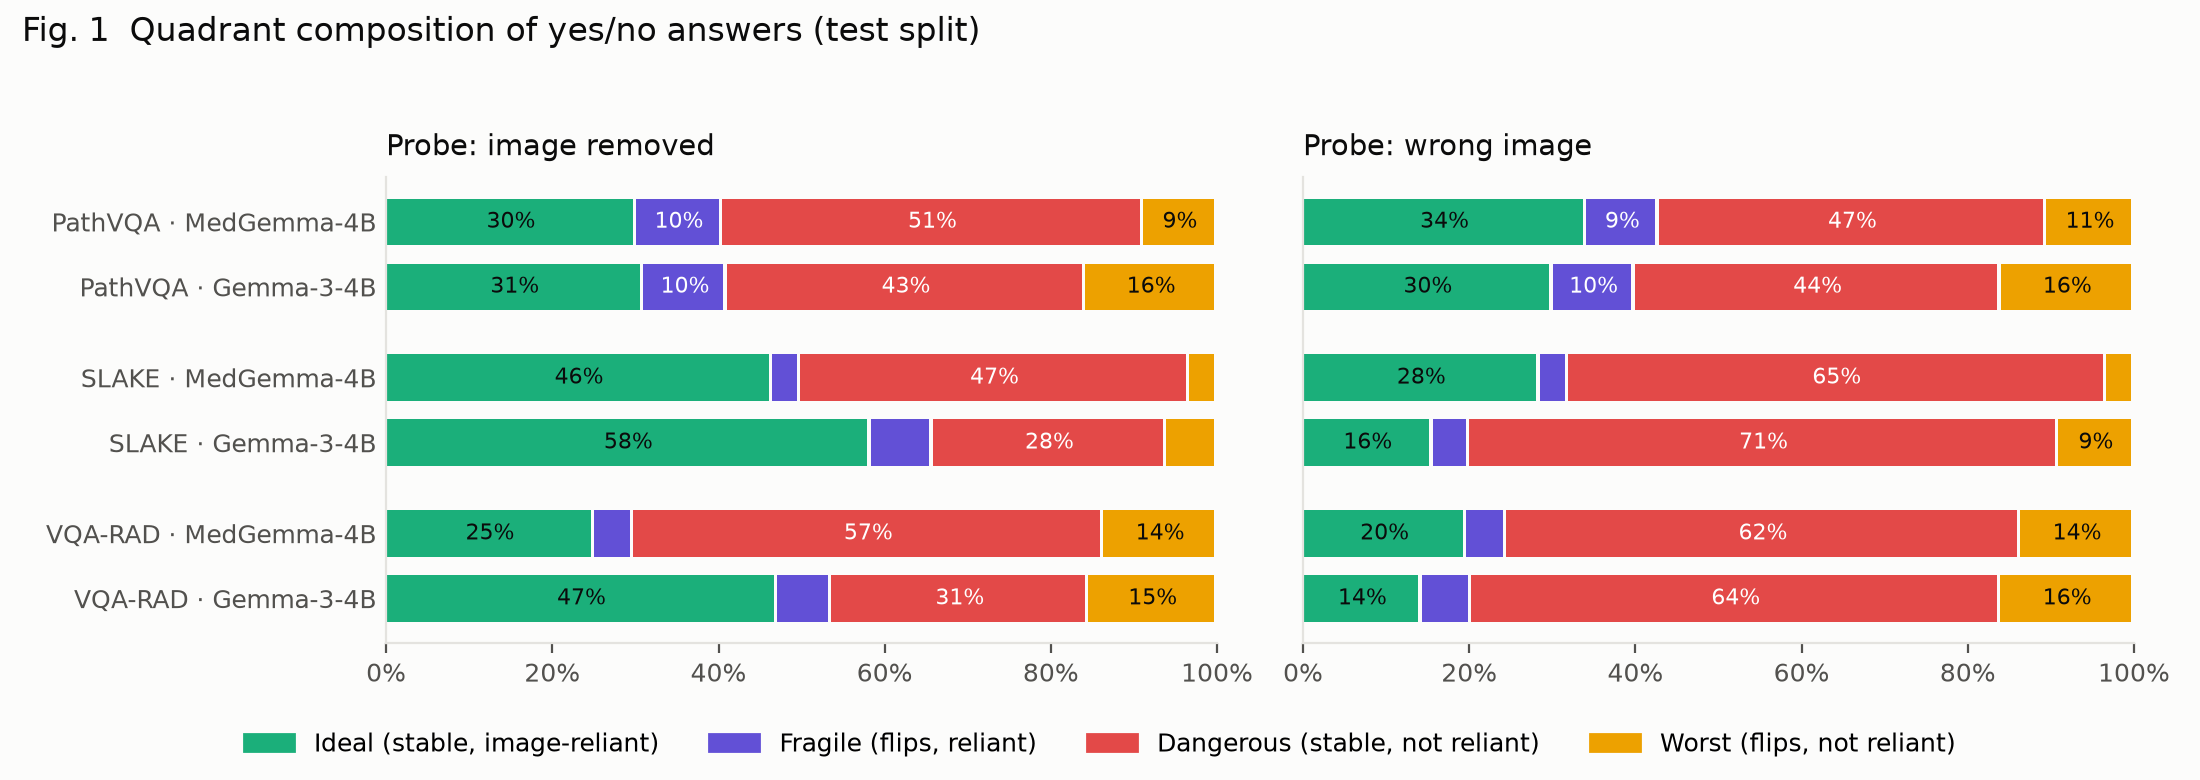
\includegraphics[width=\textwidth]{figures/fig1_quadrants.png}
\caption{Quadrant composition of yes/no answers (test). Left: reliance probed by removing the image (the
reference definition). Right: by a wrong image of the same modality. Shares are raw; on yes/no questions they
include chance agreement (\S\ref{sec:chance}).}\label{fig:quad}
\end{figure*}

Figure~\ref{fig:quad} shows the composition. Under the image-removed probe MedGemma's \dang{} share is
50.6/46.8/56.5\% (PathVQA/SLAKE/VQA-RAD), against 43.2/28.1/31.0\% for Gemma-3. Under the wrong-image probe
the two models are similar (46.6/64.7/61.9 vs.\ 44.1/70.8/63.7). The probes agree poorly: $\kappa$ between
``reliant without the image'' and ``reliant with a wrong image'' is 0.23, $-0.11$ and 0.18 for MedGemma and
0.07, 0.03 and 0.07 for Gemma-3. A \dang{} share is therefore underspecified without its probe.

\begin{figure*}[t]
\centering
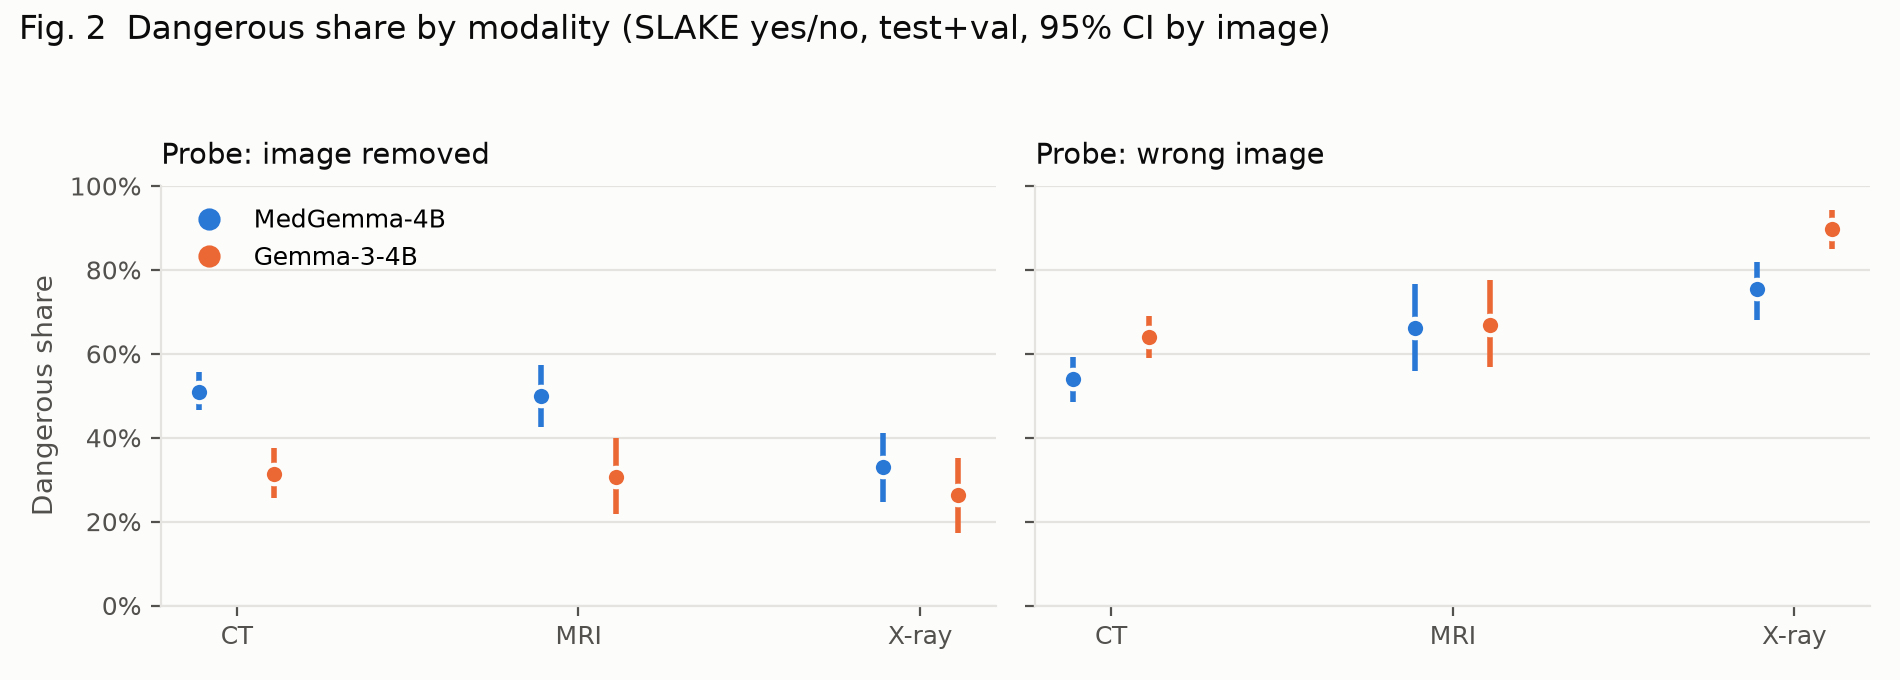
\includegraphics[width=0.86\textwidth]{figures/fig2_modality.png}
\caption{\dang{} share by modality (SLAKE yes/no, test and validation pooled as pre-specified; 95\% CIs by
image). The modality ordering reverses between probes.}\label{fig:mod}
\end{figure*}

\textbf{Modality} (Fig.~\ref{fig:mod}). With the image removed, MedGemma's \dang{} share is about 50\% for CT
(50.8\ci{46.6}{55.6}) and MRI (50.0\ci{42.6}{57.4}) and lower for X-ray (33.1\ci{24.8}{41.2}). With a wrong
image the order reverses and X-ray is the highest (75.4\%). The reversal has a mechanical cause. Where the
partner image carries the same question we can read its gold answer: \emph{all 23} chest X-ray partners had
the same correct answer (CT 58\%, MRI 60\%), so an unchanged answer there is correct, not blind. On the 35
swaps whose correct answer does change, MedGemma changes its answer 74\% of the time and Gemma-3 17\%
(post hoc, small $n$).

\subsection{Q3: Does image reliance flag wrong answers?}
\begin{figure*}[t]
\centering
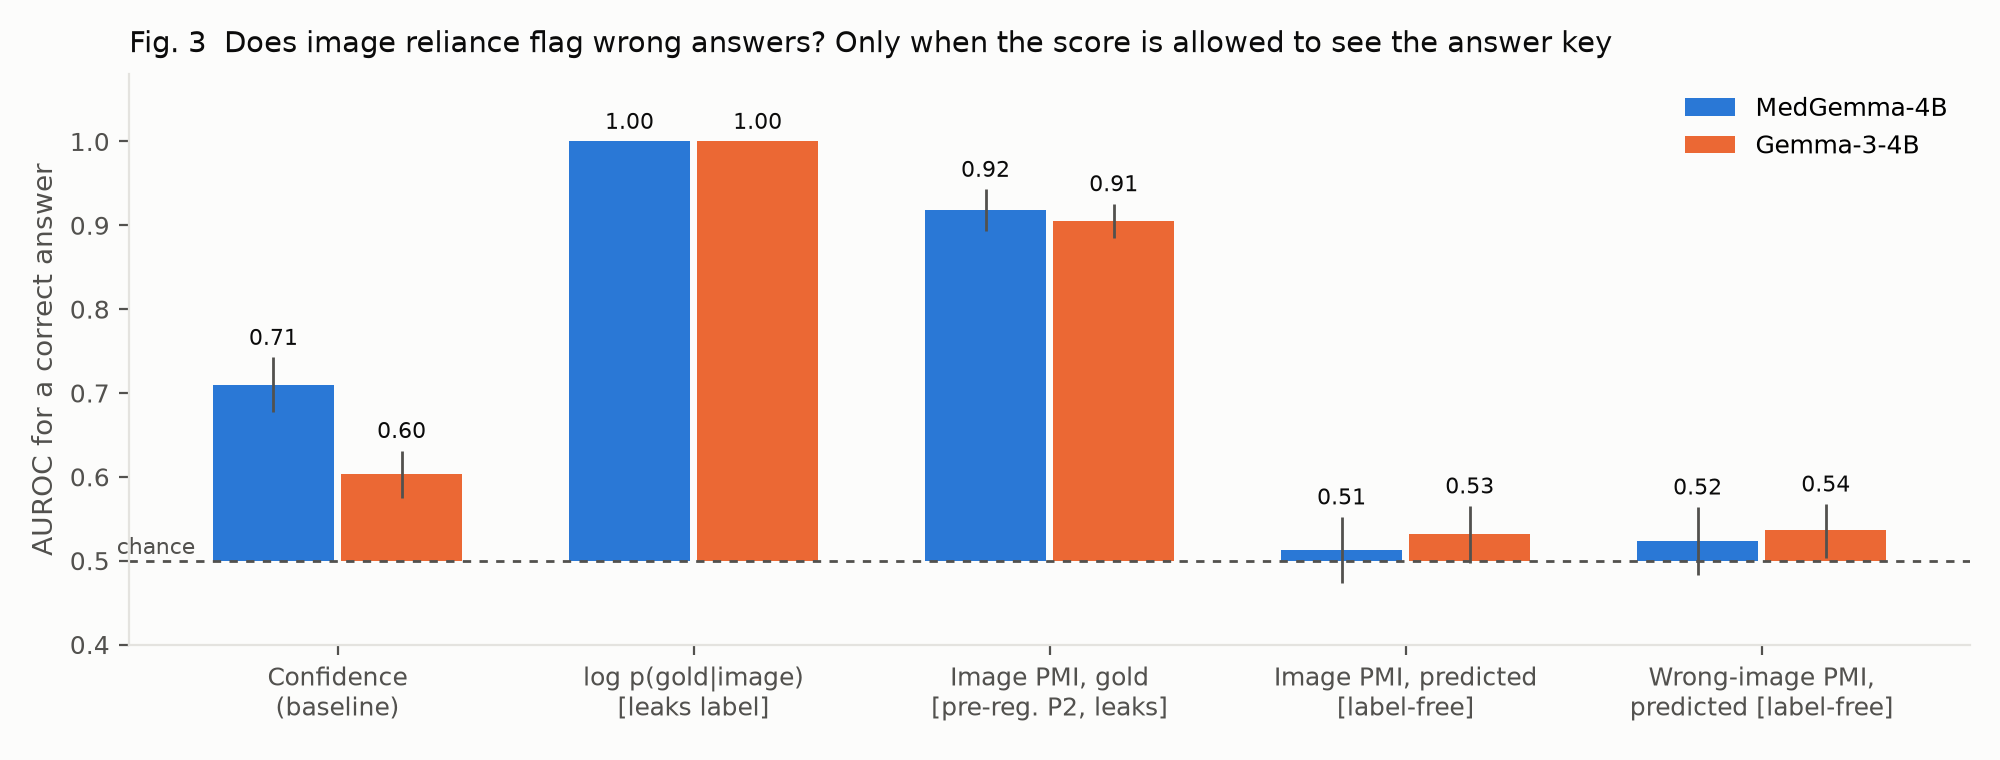
\includegraphics[width=0.92\textwidth]{figures/fig3_leakage.png}
\caption{AUROC for predicting a correct yes/no answer (test, 95\% CIs). Scores that use the gold answer
look strong because they encode it; the label-free reliance scores are at chance.}\label{fig:leak}
\end{figure*}

The pre-registered P2 is significant, $+0.209$\ci{0.161}{0.255} for MedGemma, but it is \textbf{confounded
by label leakage} (Fig.~\ref{fig:leak}). For a yes/no question the answer is correct exactly when
$\log p(y^\ast\mid I,q)>\log 0.5$, so the first term of the gold-based PMI is the answer key: on its own it
has AUROC 1.000, and the PMI inherits most of it (0.919). The deployable version uses the model's prediction
$\hat y$: label-free image PMI has AUROC \textbf{0.513}\ci{0.473}{0.552} (MedGemma) and 0.532 (Gemma-3), at
chance, and confidence beats it by 0.197\ci{0.145}{0.250} and 0.071\ci{0.026}{0.116}. The wrong-image variant
is no better (0.524, 0.536). Whether a model leaned on the image does not tell us whether it was right. The
design error is ours; the pilot's encouraging estimate had the same cause.

\subsection{Q4: What medical tuning changes}
\textbf{Abstention.} The pre-registered format check ($m\ge0.9$) failed in exactly one condition, image
removed (MedGemma 37--67\% of yes/no questions below 0.9, Gemma-3 18--76\%; with the image $\ge99.8\%$).
Free generation explains it: ``\emph{Please provide the image. I need to see the image to determine if the
larynx is present}'' (Gemma-3); ``\emph{I am unable to answer this question as I do not have access to
medical images}'' (MedGemma). This is behavior, not a bug, so we keep the pre-registered forced-choice
$P(\text{yes})$ and report abstention as an outcome (Fig.~\ref{fig:abst}). Gemma-3 abstains on 14.0, 40.6 and
50.2\% of questions (PathVQA, SLAKE, VQA-RAD), MedGemma on 9.7, 26.2 and 27.1\%; paired difference
$-11.2$\ci{-14.0}{-8.6}~points.

\begin{figure}[t]
\centering
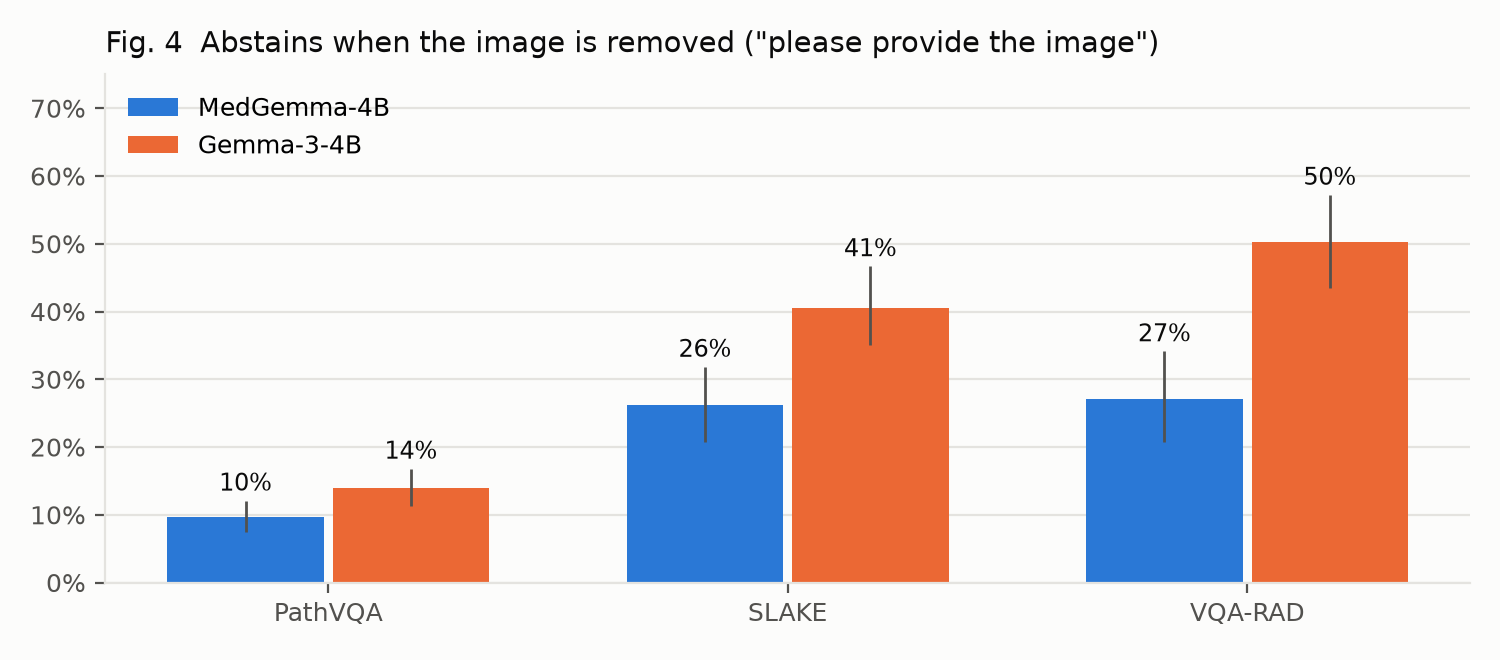
\includegraphics[width=\columnwidth]{figures/fig4_abstention.png}
\caption{Share of yes/no questions on which the model mostly does not answer yes/no when the image is
removed ($m<0.5$; 95\% CIs by image).}\label{fig:abst}
\end{figure}

\textbf{P3.} MedGemma's \dang{} share is \textbf{13.7 points higher}\ci{10.0}{17.5} ($p<0.001$; 1,012
questions, 600 images), positive in every dataset (PathVQA +7.5\ci{2.6}{12.3}, SLAKE +18.6\ci{12.2}{24.9},
VQA-RAD +25.6\ci{14.7}{36.5}) and in every cell of the sensitivity grid. Removing questions on which either
model abstains reduces it to +8.0\ci{2.9}{13.3} (both $m\ge0.9$, $n=436$) or +12.6\ci{8.1}{17.0} (both
$m\ge0.5$). Under the wrong-image probe it is $-0.7$\ci{-4.4}{3.2} (Fig.~\ref{fig:p3}).

\begin{figure*}[t]
\centering
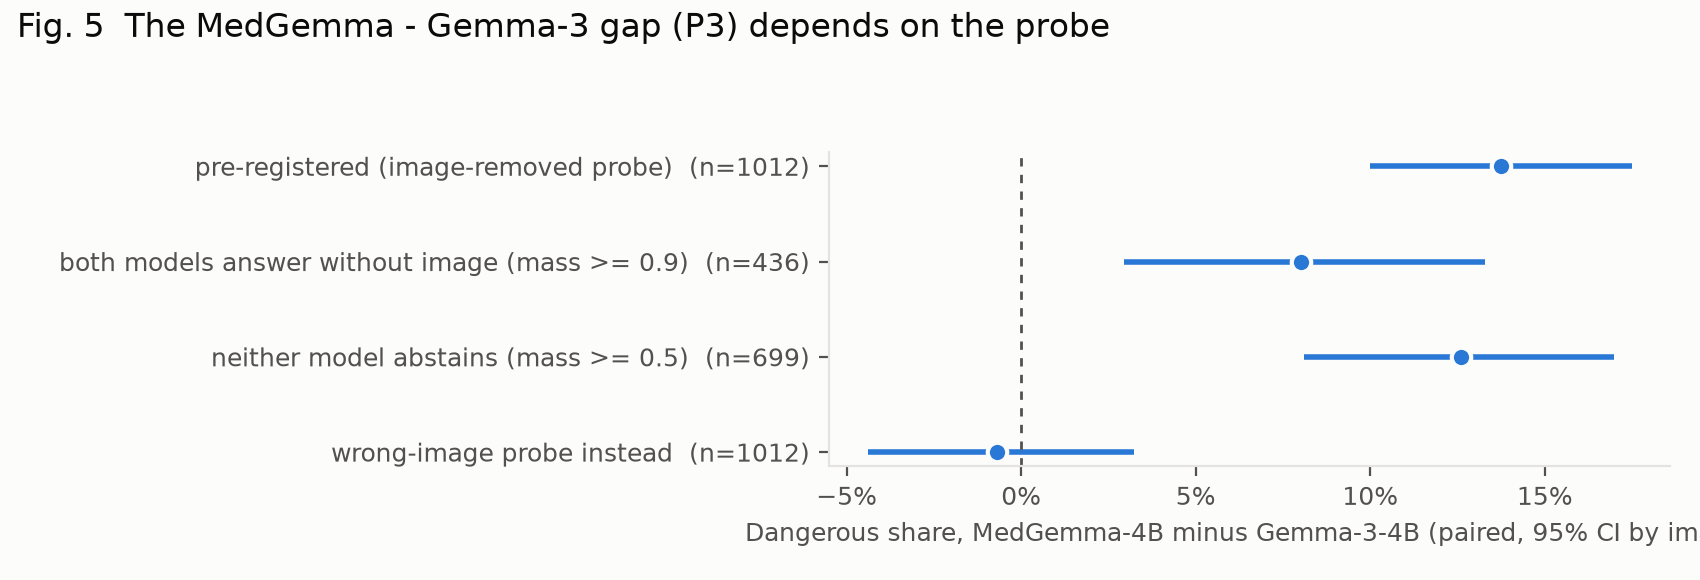
\includegraphics[width=0.72\textwidth]{figures/fig5_p3.png}
\caption{P3, the paired difference in \dang{} share (MedGemma $-$ Gemma-3), under the pre-registered
probe, after removing abstaining questions, and under the wrong-image probe.}\label{fig:p3}
\end{figure*}

\subsection{How much of \dang{} is chance?}\label{sec:chance}
An answer counts as image-independent whenever the no-image answer \emph{equals} the with-image answer,
which on yes/no questions happens often by chance. On the P3 set, MedGemma's answers are unchanged without
the image 58.6\% of the time against 49.1\% expected from its answer distributions alone (Gemma-3: 49.7\%
vs.\ 45.7\%). Combined with consistency, this gives a \textbf{chance floor of 41.5\% (MedGemma) and 35.8\%
(Gemma-3)} against observed \dang{} shares of 50.5\% and 36.8\%: Gemma-3 is at its floor and MedGemma 9 points
above it. About 6 of the 13.7 points of P3 are the difference in floors, partly because MedGemma is more
consistent (84.5\% vs.\ 78.4\% of questions), a desirable property the quadrant metric counts against it.
Corrected for chance, the effect remains: $\kappa(\text{orig},\text{noimg})=0.186$\ci{0.126}{0.250} vs.\
0.074\ci{0.022}{0.128}, $\Delta\kappa=+0.112$\ci{0.044}{0.180}, $p=0.002$.

\section{Discussion}
\textbf{The risk is missing images, not ignored ones.} With an informative image present, MedGemma uses it:
it is 18 points more accurate than Gemma-3 on SLAKE yes/no and follows answer-changing image swaps 74\% of
the time. What medical tuning adds is a willingness to answer \emph{without} the image, with answers that
beat the prior and agree with its image-based answers beyond chance. This reproduces the
\emph{consistent but dangerous} pattern reported for fine-tuned chest X-ray models~\cite{sadanandan2026consistent},
here on CT, MRI, X-ray, radiology and pathology. In deployment the failure would appear when an image fails
to load, is the wrong study, or is uninformative, and the model answers confidently anyway.

\textbf{Recommendations for reliance audits.} (1) Report the \dang{} share with its chance floor or as
$\kappa$; on balanced yes/no data a model whose blind answers are pure noise is about 50\% ``not reliant''.
(2) Use more than one probe and report their agreement; removing the image measures willingness to answer
blind, a wrong image measures sensitivity to content, and the latter needs answer-changing swaps.
(3) Never evaluate a reliance score with the gold answer inside it. (4) Treat abstention without the image as
a desirable behavior, not a format failure.

\section{Limitations}
One audited model and one control are not a population of models. SLAKE is in MedGemma's training data
(split unstated). Abstention is inferred from first-token mass and confirmed on a sample by free generation,
not annotated per question. The partner-gold analysis covers only the 112 swaps where the partner image
carries the same question. Paraphrase equivalence was judged by an LLM, not by clinicians.
\textcolor{red}{[PENDING: human spot-check of 50 accepted pairs; insert agreement here once rated.]} PathVQA questions are auto-generated and
often ungrammatical. All 330 pilot questions used to tune the design are inside the evaluation set;
excluding them leaves every conclusion unchanged (P1a +6.3\ci{2.4}{10.6}, P3 +12.9\ci{8.9}{17.1}). Benchmark
VQA is not clinical use, and nothing here is a clinical claim.

\section{Implementation Details}
\textbf{Pipeline.} A Python package (\texttt{medvlm}) with a command-line interface:
\texttt{prepare} (download, deterministic sampling, SHA-checked images), \texttt{paraphrase} (generation plus
rule and judgment validation, fail-closed), \texttt{pipeline} (resumable inference in parts with checkpoint
analysis), \texttt{analyze}, \texttt{compare} and \texttt{posthoc} (all tables and figures here). Configs layer
base, profile, model and hardware settings. Each job is one (question, condition) pair keyed by ID, so
interrupted runs resume without recomputation, and every run records its config, commit and library versions.

\textbf{Inference.} PyTorch 2.11 and Hugging Face Transformers 5.19, bf16, SDPA attention, one RTX 4080
SUPER (16\,GB). A full run is 18,896 calls per model at 0.23\,s per call (about 75 minutes, 8.2\,GB peak).
During pre-flight we found that in bf16 the \emph{batch size} changes teacher-forced log-probabilities by up
to 1.09 nats (median 0.17) even with identical, unpadded inputs, while $P(\text{yes})$ changes by at most
0.008. An fp32 output head did not remove it, so the cause is inside the network. All runs therefore use
batch size 1, which costs about 1.5$\times$ throughput. A regression check reproduced the T4 pilot on the new
GPU (98.5\% identical answers, mean $|\Delta P(\text{yes})|=0.004$).

\textbf{Testing.} 91 unit tests and 7 real-model tests cover, among others, scoring edge cases, paraphrase
rules (including each failure class found in the audit), batching equivalence, crash-safe resume, the
coverage of the clustered bootstrap (by simulation), the test-split restriction of P3, and the two pitfalls
above (label leakage of gold-based scores, chance agreement of $\kappa$).

\section{Conclusion}
Medical tuning makes a small VLM better at looking and more willing to answer without looking. The second
effect produces more answers that look trustworthy and do not depend on the image, across modalities.
Measuring this reliably requires chance correction, more than one probe, and scores that never see the
answer key. The pre-registered score we designed to catch these answers failed that last test.

{\small
\bibliographystyle{plainnat}
\bibliography{refs}
}

\appendix
\onecolumn
\section{Paraphrase equivalence rubric}\label{app:rubric}
A pair is \textbf{accepted} only if it asks exactly the same thing, so the correct answer cannot differ.
Allowed: perception framing (``can X be seen'', ``is X visible'', ``can X be seen to be enlarged''), exact
synonyms (clavicle/collarbone, encephalon/brain, intravenous contrast/dye), reordering. \textbf{Rejected}:
a fact turned into a possibility or capability (``Is the heart enlarged?''$\to$``Can the heart be
enlarged?''); a broadened or narrowed term (mass$\to$lesion, organs$\to$structures, digestive system$\to$GI
tract, skull fracture$\to$cranial injury); a changed scope or presupposition (``Do the organs exist in X''$\to$
``Are there organs in X''); added qualifiers, findings or modality (``bilaterally'', ``on imaging studies'',
``radiograph''); a reversed or changed relation (``does A show B''$\to$``is A associated with B'', ``mass lateral
to X''$\to$``X lateral to mass''); antonyms (healthy$\leftrightarrow$unhealthy, coronal$\to$transverse); two
questions in one; malformed text. Rejection reasons by class: relation 447, term 364, modal 106, added
content 102, organ$\to$structure 47, generic collapse 30, polarity 19, scope 9 (plus template-pass rejections).

\section{Deviations from the pre-registration}\label{app:dev}
\begin{center}\small
\begin{tabular}{p{0.28\textwidth}p{0.66\textwidth}}
\toprule
Change & Reason and effect\\
\midrule
Batch size 1 for all runs & bf16 batching shifts teacher-forced log-probabilities by up to 1.09 nats; decided before the main run.\\
Paraphrase validator v2/v3, \emph{plain} style excluded, full equivalence screen, template styles & Audit acceptance below the pre-specified 85\% line; decided before the main run.\\
Format stop-the-line rule triggered (image removed only) & Model behavior (abstention), not a pipeline error; forced-choice $P(\text{yes})$ kept, abstention reported as an outcome, P1/P3 re-estimated without abstaining questions.\\
P2 not interpreted & Gold-conditioned score leaks the label; label-free variant reported alongside.\\
P3 restricted to the test split & Analysis bug pooled the validation split ($+14.1$, $n=1{,}315$); fixed to the pre-registered set ($+13.7$, $n=1{,}012$).\\
Chance-corrected P3 ($\kappa$) & The \dang{} share has a chance floor on yes/no; added after the run, reported next to the raw estimate.\\
Partner-gold check, no-pilot re-estimation & Post-hoc robustness checks; exploratory.\\
\bottomrule
\end{tabular}
\end{center}

\end{document}
